% vim: set textwidth=78 autoindent:

%\subsection{Decorations Plugins}
\subsection{Extensions de décoration}

% when the revision of a section has been finalized, 
% comment out the following line:
% \updatedisclaimer

%The Decorations Plugins includes the Copyright Label Plugin, the North 
%Arrow Plugin and the Scale Bar Plugin. They are used to ``decorate'' the 
%map by adding cartographic elements.
Les extensions de décoration comprennent les extensions Étiquette de Copyright, 
Flèche Nord et Échelle Graphique. Elles sont destinées à "habiller" la carte en
ajoutant des éléments cartographiques.

%\subsubsection{Copyright Label Plugin}
\subsubsection{L'extension Etiquette de Copyright}

%The title of this plugin is a bit misleading - you can add any random text to the map.
Le nom de cette extension est un peu trompeur, vous pouvez en réalité ajouter
n'importe quel type de texte à la carte.

%\begin{figure}[ht]
%   \begin{center}
%   \caption{Copyright Label Plugin \nixcaption}\label{fig:copyright}\smallskip
%   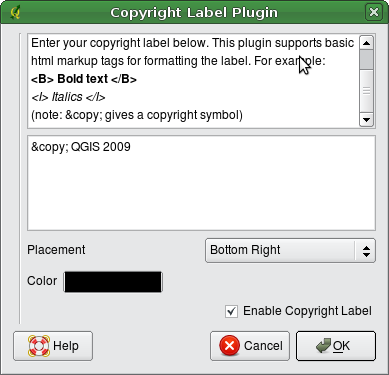
\includegraphics[clip=true, width=8cm]{copyright}
%\end{center}  
%\end{figure}
\begin{figure}[ht]
   \begin{center}
   \caption{L'extension Etiquette de Copyright \nixcaption}\label{fig:copyright}\smallskip
   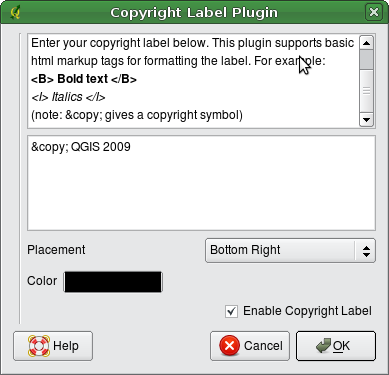
\includegraphics[clip=true, width=8cm]{copyright}
\end{center}  
\end{figure}

%\begin{enumerate}
%\item Make sure the plugin is loaded
%\item Click on \mainmenuopt{Plugins} > \dropmenuopt{Decorations} > \dropmenuopttwo{copyright_label}{Copyright Label} or use the \toolbtntwo{copyright_label}{Copyright Label} button from the Toolbar.
%\item Enter the text you want to place on the map. You can use HTML as
%  shown in the example
%\item Choose the placement of the label from the \selectstring{Placement}{Bottom Right} drop-down box
%\item Make sure the \checkbox{Enable Copyright Label} checkbox is checked
%\item Click \button{OK} 
%\end{enumerate}
\begin{enumerate}
\item Assurez-vous d'avoir activé l'extension
\item Appuyez sur \mainmenuopt{Extension} > \dropmenuopt{Décorations} > \dropmenuopttwo{copyright_label}{Etiquette de Copyright} ou utilisez le bouton \toolbtntwo{copyright_label}{Etiquette de Copyright} directement depuis la barre d'outils.
\item Entrez le texte que vous souhaitez placer sur la carte. Vous pouvez
  utiliser certaines balises HTML comme montrées dans l'exemple
\item Choisissez la position de l'étiquette avec la liste de choix déroulante \selectstring{Placement}{Coin Inférieur Droit}
\item Assurez-vous que la case \checkbox{Activer l'étiquette du Copyright} soit cochée
\item Appuyez sur \button{OK} 
\end{enumerate}

%In the example above (default) places a copyright symbol followed by the date in the 
%lower right hand corner of the map canvas.
L'exemple ci-dessus (par défaut) permet et placer et d'afficher un symbole de
copyright suivi de la date dans le coin inférieur droit de la carte.

%\subsubsection{North Arrow Plugin}
\subsubsection{L'extension Flèche Nord}

%The North Arrow plugin places a simple north arrow on the map canvas. At
%present there is only one style available. You can adjust the angle of the
%arrow or let QGIS set the direction automatically. If you choose to let
%QGIS determine the direction, it makes its best guess as to how the arrow
%should be oriented. For placement of the arrow you have four options, 
%corresponding to the four corners of the map canvas.
L'extension Flèche Nord place une simple rose des vents sur la carte. Un seul
style est disponible pour le moment. Vous pouvez ajuster l'angle de la flèche 
ou laisser QGIS déterminer automatiquement la direction. Si vous faites ce 
dernier choix, QGIS essaiera de calculer la meilleure orientation de la flèche.
Quatre options sont disponibles pour la position de la flèche, qui correspondent
au quatre coins de la carte du projet.

%\begin{figure}[ht]
%   \begin{center}
%   \caption{North Arrow Plugin \nixcaption}\label{fig:north_arrow}\smallskip
%   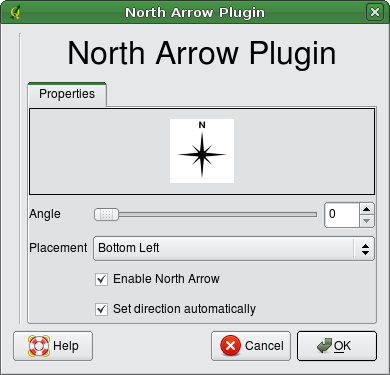
\includegraphics[clip=true, width=8cm]{north_arrow_dialog}
%\end{center}  
%\end{figure}
\begin{figure}[ht]
   \begin{center}
   \caption{L'extension Flèche Nord \nixcaption}\label{fig:north_arrow}\smallskip
   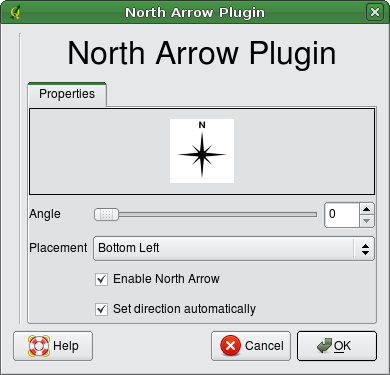
\includegraphics[clip=true, width=8cm]{north_arrow_dialog}
\end{center}  
\end{figure}

%\subsubsection{Scale Bar Plugin}
\subsubsection{L'extension Échelle Graphique}

%The Scale Bar plugin adds a simple scale bar to the map canvas. You
%control the style and placement, as well as the labeling of the bar. 
L'extension Échelle Graphique ajoute une simple échelle graphique à la carte du
projet.
Vous pouvez en contrôler le style, la position, ainsi que l'apparence.

%QGIS only supports displaying the scale in the same units as your map frame. So
%if the units of your layers are in meters, you can't create a scale bar in
%feet. Likewise if you are using decimal degrees, you can't create a scale
%bar to display distance in meters.
Dans QGIS, l'affichage de l'échelle graphique ne peut se faire que dans la même 
unité que le projet de la carte. Ainsi, si l'unité de vos couches est en mètres, 
vous ne pouvez pas créer une échelle graphique en pieds. De la même manière, si 
vous utilisez les degrés décimaux, vous ne pouvez pas créer une échelle 
graphique qui affiche les distances en mètres.

%To add a scale bar:
Pour ajouter une échelle graphique :

%\begin{enumerate}
%\item Click on \mainmenuopt{Plugins} > \dropmenuopt{Decorations} > \dropmenuopttwo{scale_bar}{Scale Bar} or use the \toolbtntwo{scale_bar}{Scale Bar} button from the Toolbar.
%\item Choose the placement from the \selectstring{Placement}{Bottom Left} drop-down list
%\item Choose the style from the \selectstring{Scale bar style}{Tick Down} list
%\item Select the color for the bar \selectcolor{Color of bar}{black} or use the default black color
%\item Set the size of the bar and its label \selectnumber{Size of bar}{30 degrees}
%\item Make sure the \checkbox{Enable scale bar} checkbox is checked
%\item Optionally choose to automatically snap to a round number when the
%  canvas is resized \checkbox{Automatically snap to round number on resize}
%\item Click \button{OK} 
%\end{enumerate} 
\begin{enumerate}
\item Appuyez sur \mainmenuopt{Extension} > \dropmenuopt{Décorations} > \dropmenuopttwo{scale_bar}{Echelle graphique} ou utilisez le bouton \toolbtntwo{scale_bar}{Echelle graphique} depuis la barre d'outils.
\item Choisissez la position de l'échelle à l'aide de la liste déroulante \selectstring{Placement}{Coin Inférieur Gauche}.
\item Choisissez le style de l'échelle à l'aide de la liste déroulante \selectstring{Scale bar style}{Marquage Inférieur}.
\item Choisissez la couleur de l'échelle \selectcolor{Color of bar}{black} ou utilisez le noir par défaut.
\item Définissez la taille et l'étiquette de l'échelle \selectnumber{Size of bar}{30 degrés}
\item Assurez-vous que la case \checkbox{Activer l'échelle graphique} soit cochée.
\item Optionnellement, vous pouvez choisir d'arrondir automatiquement l'échelle 
  à chaque changement du niveau de zoom \checkbox{Arrondir automatiquement lors du changement de zoom}
\item Appuyez sur \button{OK} 
\end{enumerate} 

%\begin{figure}[ht]
%   \begin{center}
%   \caption{Scale Bar Plugin \nixcaption}\label{fig:scale_bar}\smallskip
%   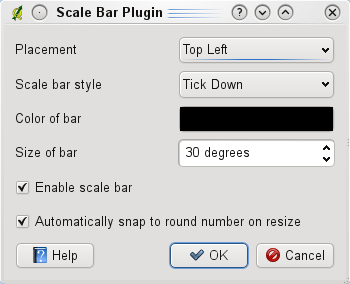
\includegraphics[clip=true, width=8cm]{scale_bar_dialog}
%\end{center}  
%\end{figure}
\begin{figure}[ht]
   \begin{center}
   \caption{L'extension Échelle Graphique \nixcaption}\label{fig:scale_bar}\smallskip
   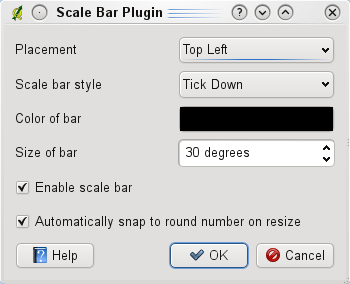
\includegraphics[clip=true, width=8cm]{scale_bar_dialog}
\end{center}  
\end{figure}

%\begin{Tip}\caption{\textsc{Plugins Settings Saved to Project}}\index{plugins settings}
%\qgistip{When you save a .qgs project, any changes you have made to NorthArrow, ScaleBar and Copyright plugins will be saved in the project and restored nexttime you load the project.}
%\end{Tip}
\begin{Tip}\caption{\textsc{Sauvegarde des paramètres de l'extension avec le projet}}\index{plugins settings}
\qgistip{Lorsque vous sauvegardez un projet QGIS en .qgs, chaque changement que 
vous avez appliqué aux extensions Flèche Nord, Échelle Graphique et Étiquette 
de Copyright sera sauvegardé avec le projet et restauré au prochain chargement 
de celui-ci.}
\end{Tip}
